% TEMPLATE for Usenix papers, specifically to meet requirements of
%  USENIX '05
% originally a template for producing IEEE-format articles using LaTeX.
%   written by Matthew Ward, CS Department, Worcester Polytechnic Institute.
% adapted by David Beazley for his excellent SWIG paper in Proceedings,
%   Tcl 96
% turned into a smartass generic template by De Clarke, with thanks to
%   both the above pioneers
% use at your own risk.  Complaints to /dev/null.
% make it two column with no page numbering, default is 10 point

% Munged by Fred Douglis <douglis@research.att.com> 10/97 to separate
% the .sty file from the LaTeX source template, so that people can
% more easily include the .sty file into an existing document.  Also
% changed to more closely follow the style guidelines as represented
% by the Word sample file. 

% Note that since 2010, USENIX does not require endnotes. If you want
% foot of page notes, don't include the endnotes package in the 
% usepackage command, below.

% This version uses the latex2e styles, not the very ancient 2.09 stuff.
\documentclass[letterpaper,twocolumn,10pt]{article}
\usepackage{usenix,epsfig,endnotes}
\usepackage{color}
\usepackage{colortbl}

\newcommand{\jc}[1]{{\footnotesize\color{red}[JC: #1]}}


\begin{document}

%don't want date printed
\date{}

%make title bold and 14 pt font (Latex default is non-bold, 16 pt)
\title{SDCDN: A Control Plane for Content Delivery Networks}

%for single author (just remove % characters)
\author{
{\rm Your N.\ Here}\\
Your Institution
\and
{\rm Second Name}\\
Second Institution
% copy the following lines to add more authors
% \and
% {\rm Name}\\
%Name Institution
} % end author

\maketitle

% Use the following at camera-ready time to suppress page numbers.
% Comment it out when you first submit the paper for review.
\thispagestyle{empty}


\subsection*{Abstract}
Content delivery networks (CDN) and overlay networks count for most of today's Internet traffic and have large impact on performance of applications (e.g., video streaming and web) that rely on them. 
Traditionally, these networks are based on distributed, rather than centralized protocols, which works more resilient and responsive in large geo-distribuetd networks. However, the trend of growing traffic volume and demands for high quality experience and that of global control planes for application call for a logically centralized architecture of CDNs and overlay networks at large where servers are coordinated in a global scale. 

To address this, we presents software-defined CDN (SDCDN), a logically centralized architecture for CDNs and, in particular, Live streaming. It is similar in spirit to software-defined networks (SDN), but differs in several key aspects. As a design choice, we argue that neithor fully centralization (i.e, SDN) nor fully decentralization (i.e., current CDN) is most desirable for CDN control plane. Instead, a careful division of functionalities between distributed servers and centralized controllers is needed to achieve both performance benefits of global coordination and faster recovery from failures. 

\section{Introduction}

\begin{itemize}
	\item CDNs are expected to carry more traffic. 
	\item Today's CDN architecture is highly distributed. With expended capacity it is also needed to have a globally coordinated control plane. The CDN performance will benefit from such control plane in three aspects: coordinated resource allocation and recovery from failure and simplified optimization for application goals. 
	\item Meanwhile, it has two fundamental challenges resulting from its overlay nature.
	\begin{itemize}
		\item Long propagation delay
		\item Multiple controller consistency
	\end{itemize}
	\item We present SDCDN that addresses the challenges by leveraging a unique opportunity of overlay networks -- flexibility of individual node. Instead of implementing a fully centralized control plane or pushing all control functionalities to centralized controllers, our control plane resides in both controller, called global control process, and distributed nodes called local control process. The two control processes run in different time scales.
\end{itemize}


\section{Motivation}
\begin{comment}
\subsection{Why centralization?}
\begin{itemize}
	\item Like in traditional SDN argument, a centralized control platform enables the development of flexible, reliable and feature-richer network control plane.
	\item Centralization enables global coordination of resources to optimize for complex application goal. Use example.
	\item Centralization enables better recovery and convergence in disruptive/congested networks. Use example.
\end{itemize}

\subsection{Why not fully centralized?}
\begin{itemize}
	\item Longer propagation delay than in LAN/WAN. \jc{need measurement data to support this.}
	\item Long delay to get a converged network view under large-area disruption/congestion. \jc{need measurement data to support this.}
\end{itemize}

\subsection{Two level control plane design}
Present our design of control plane that runs both in local node and controller.
\end{comment}





\begin{figure}[t]
\centering
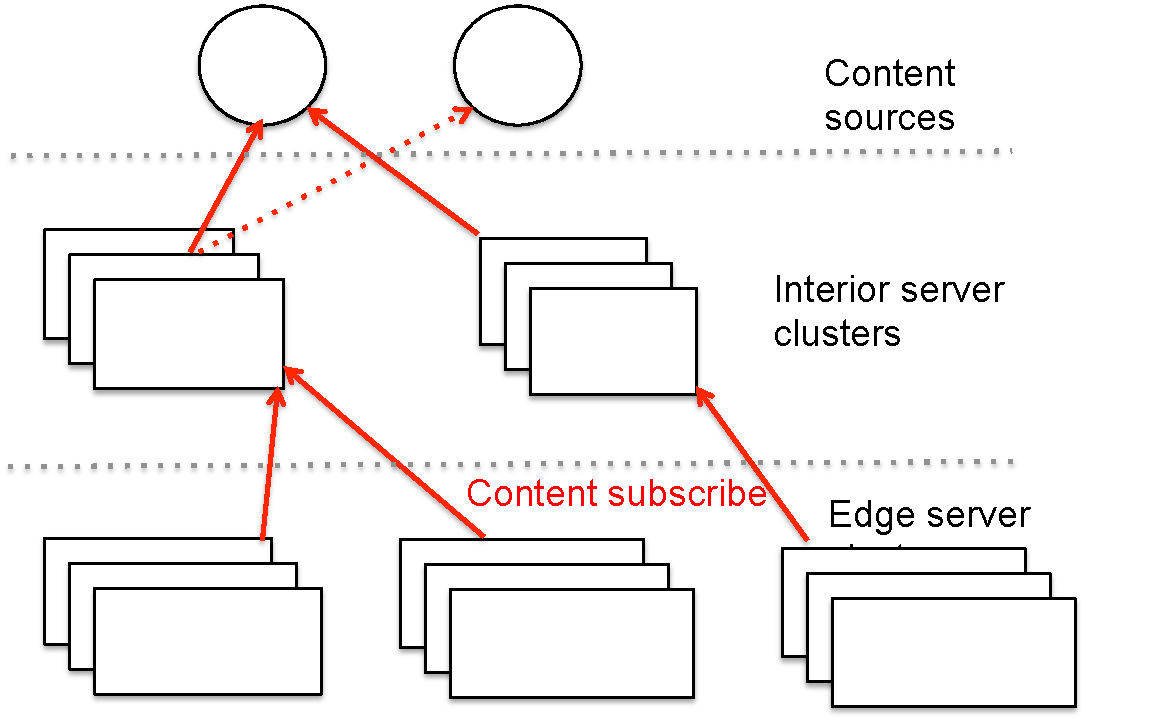
\includegraphics[width=0.90\columnwidth]{figures/cdn}
\caption{Structure of live content distribution in a CDN~\cite{akamai-live}.}
\label{fig:cdn}
\end{figure}

\captionsetup{font=small}

\begin{figure}[t]
\centering
\begin{minipage}[b]{0.32\columnwidth}
  \centering
  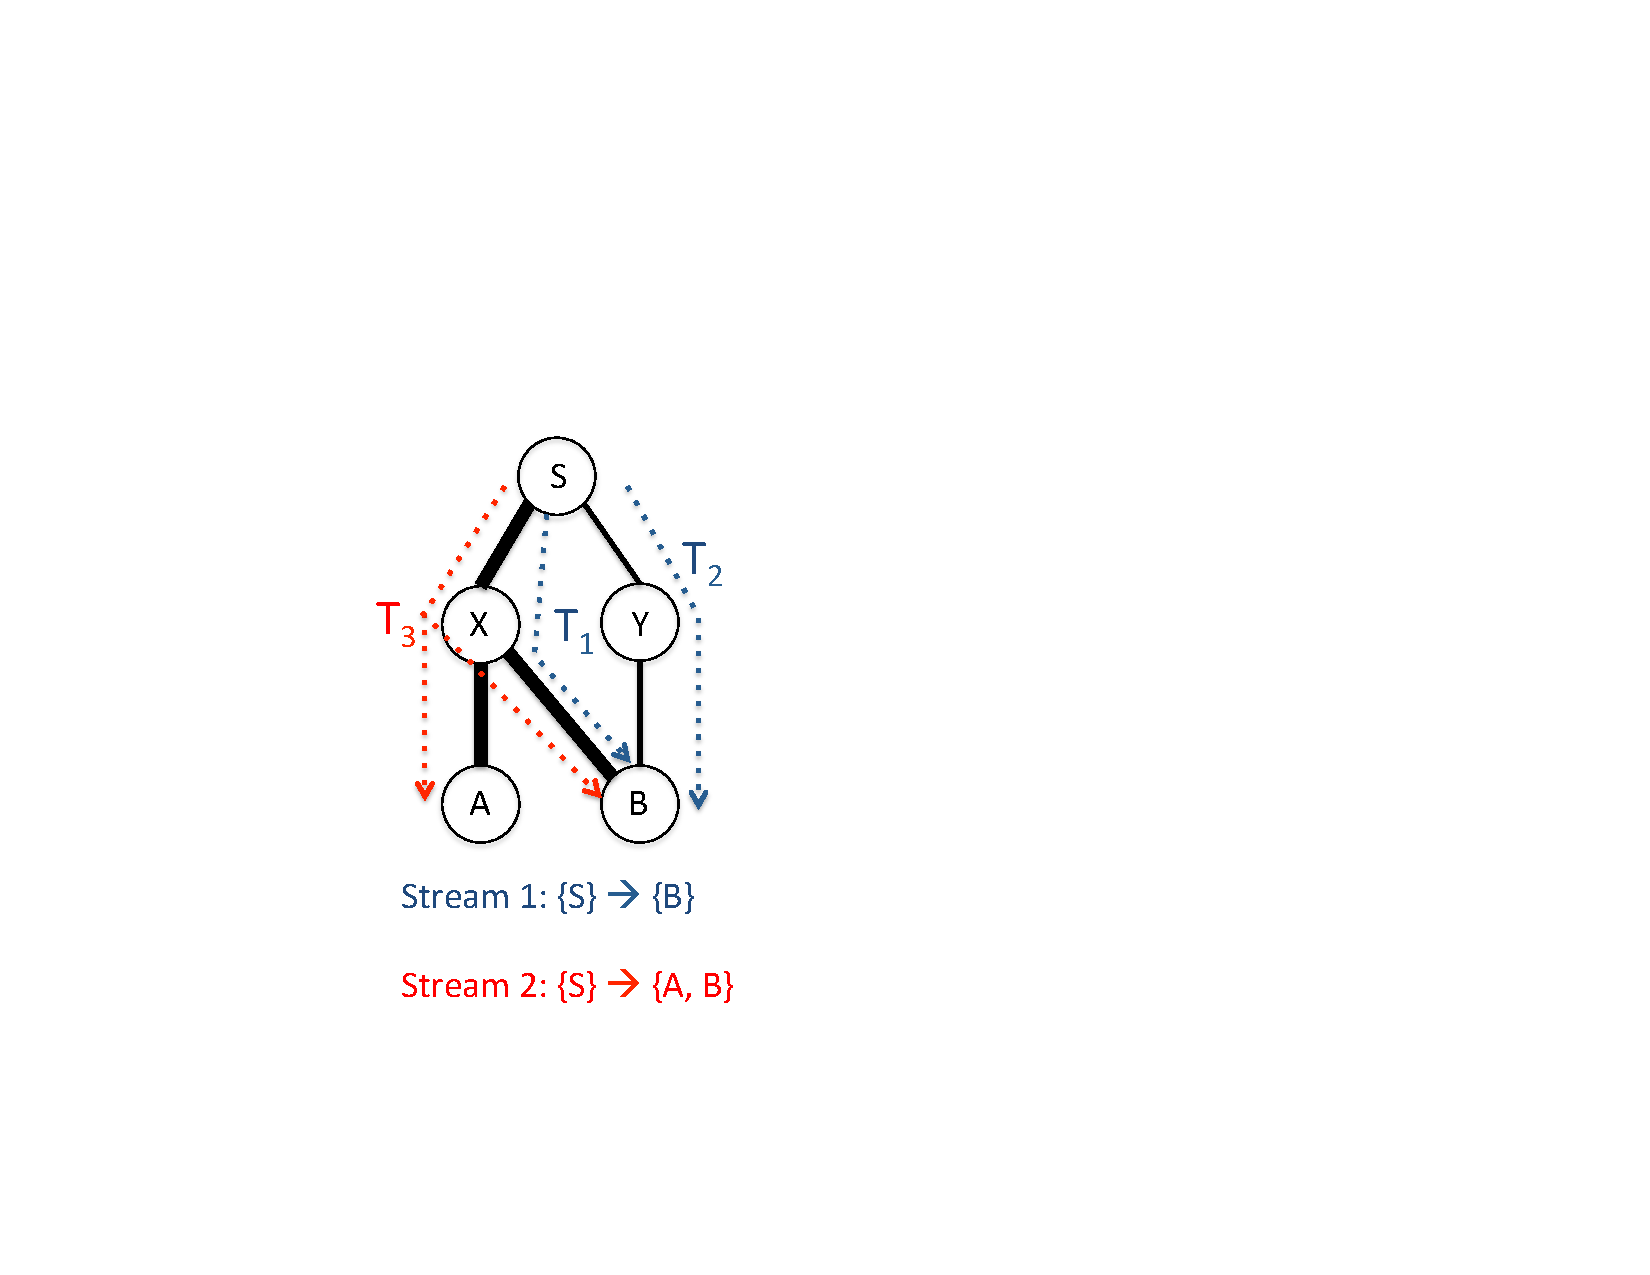
\includegraphics[scale=.40]{figures/toy-alltrees}
  \caption{\\Example Scenario}
  \label{fig:toy-alltrees}
\end{minipage}
\begin{minipage}[b]{0.32\columnwidth}
  \centering
  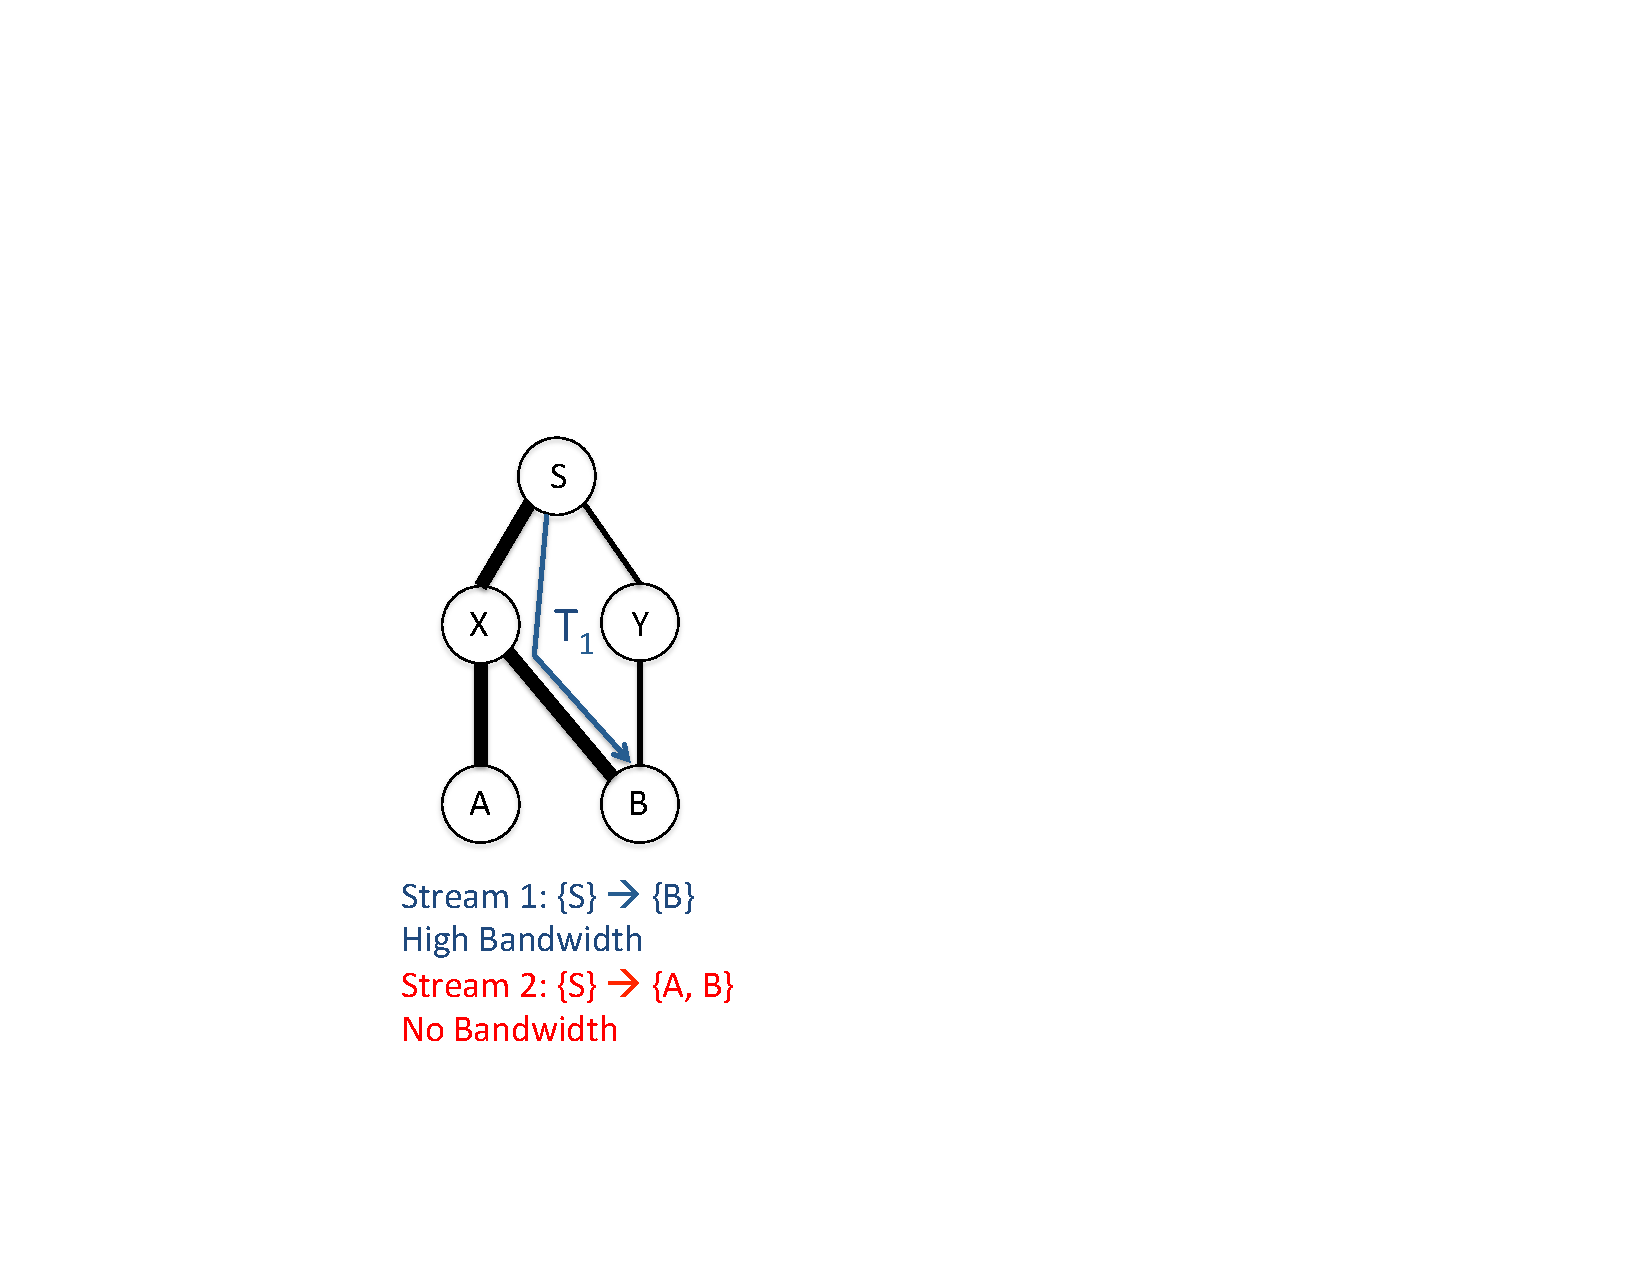
\includegraphics[scale=.40]{figures/toy-current}
  \caption{\\Current CDN}
  \label{fig:toy-current}
\end{minipage}
\begin{minipage}[b]{0.32\columnwidth}
  \centering
  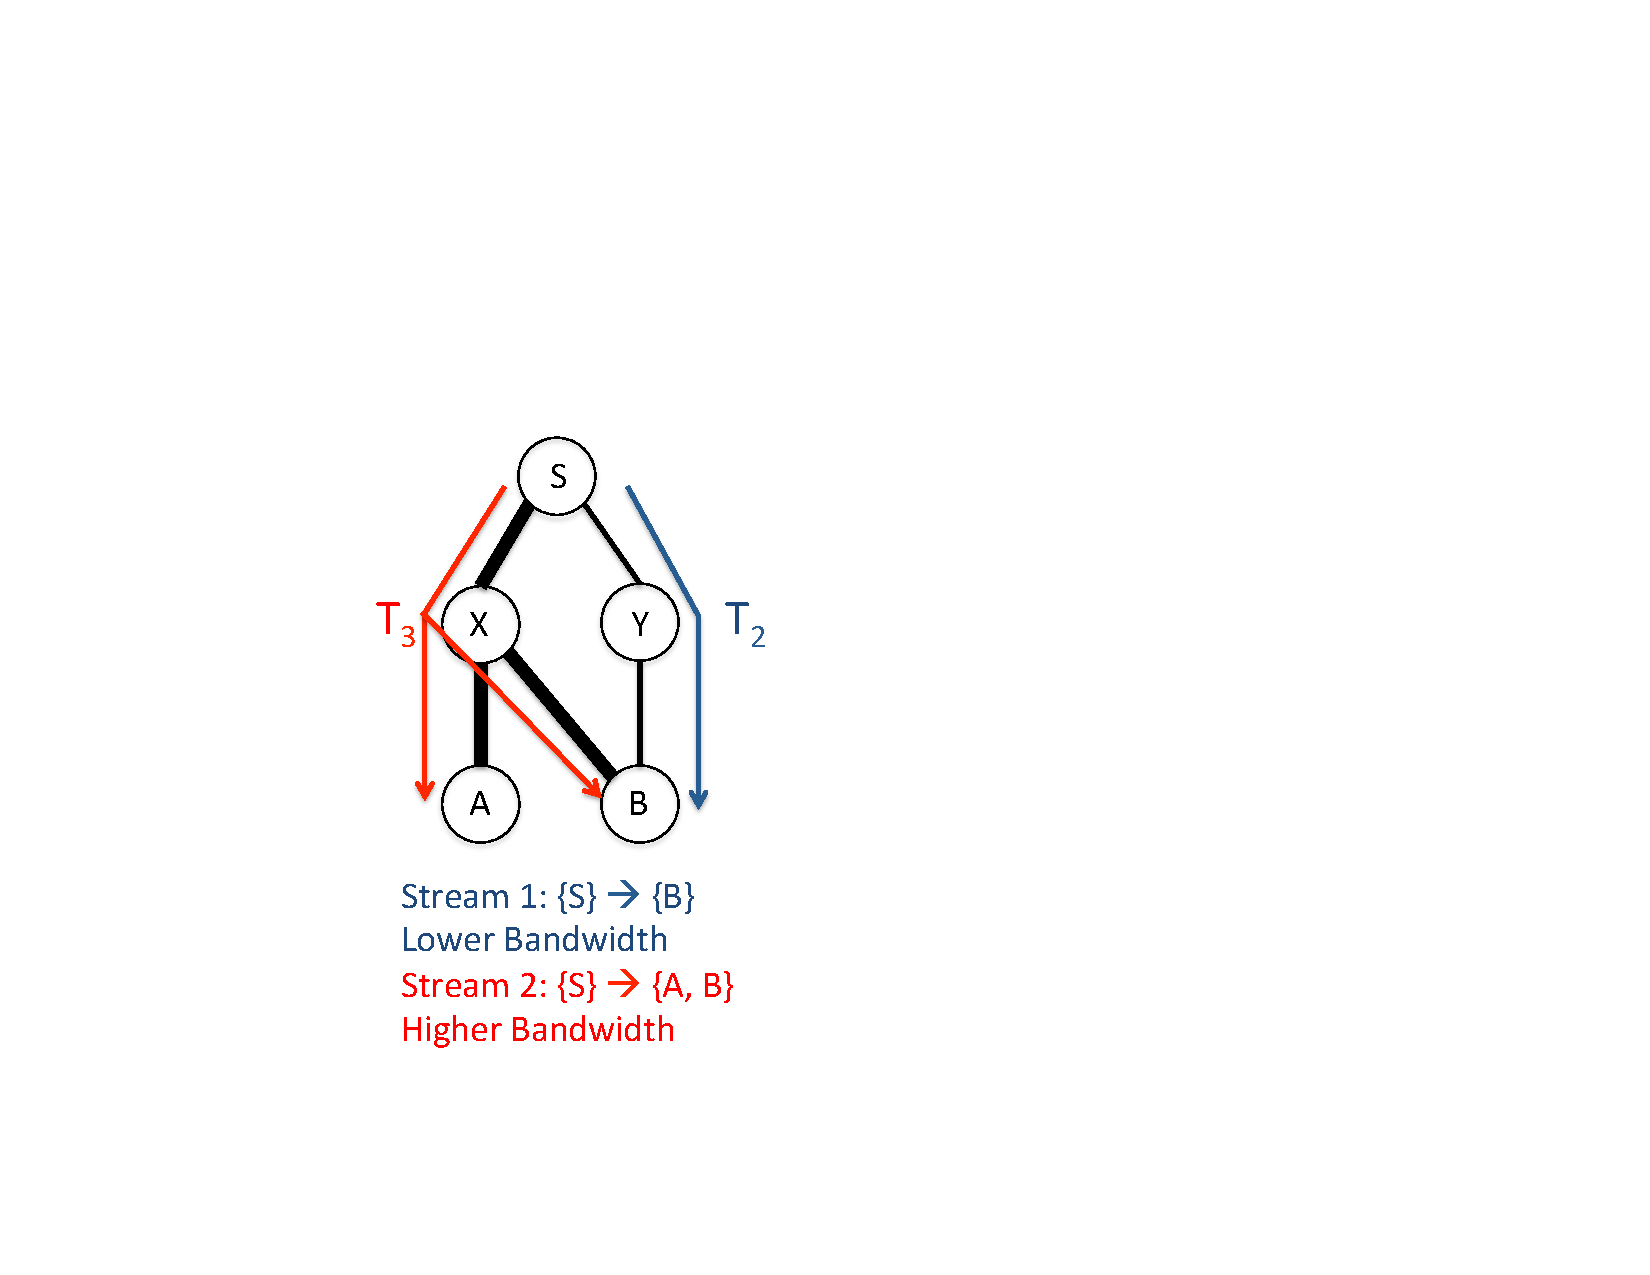
\includegraphics[scale=.40]{figures/toy}
  \caption{\\SDN+CDN}
  \label{fig:toy}
\end{minipage}
\end{figure}

\subsection{Current state-of-the-art}

Figure~\ref{fig:cdn} presents the high-level structure of a CDN's internal
video delivery system as described in ~\cite{akamai-live}. A set of co-located
servers form a cluster.
%Communication within the cluster can use multicast as it
%is often within a single LAN\@.  
Clients' video requests are directed to edge servers.  When an edge server gets
a request from a client, it subscribes to the content from one of the interior
clusters. The internal clusters are geo-distributed in well-provisioned
locations.  These servers directly receive content from the content sources (e.g., video origins).

The set of internal nodes are determined manually~\cite{akamai-live}, and thus
the distribution structure forms a rather rigid three-tiered hierarchy~\cite{spaa,akamai-live}.
Furthermore, the system does not have the knowledge of global resources, as distribution trees
are formed independently without much coordination.
For example, even though edge servers use multiple path from a content source
when the stream quality deteriorates, each edge server independently selects how many paths to use
without any coordination~\cite{akamai-live}.

\jc{need to define terminologies somehow: chunk, bitrate, stream, video server, origin}

\subsection{Why centralized control?}

Figure~\ref{fig:toy-alltrees} illustrates a simple example that 
demonstrates uncoordinated decision making leads to sub-optimal resource allocation. 
Links shown in bold are higher capacity than the non-bold links. 
%We wish to deliver two video streams (Stream 1 and Stream 2) through the network, both
%originating from source \emph{S}. 
There are two video streams (Stream 1 and 2) originating from source  \emph{S}.
The goal is to deliver Stream 1 to \emph{B} and Stream 2 to both \emph{A} and \emph{B}.

Three possible distribution trees exist in this configuration: $T_1$,
$T2$ and $T3$. 
Among the three only $T1$ and $T_2$ are useful for delivering Stream 1 to \emph{B}.
%However, $T_1$ provides higher bandwidth.
%$T_3$ is the only tree useful to Stream 2.
Now assume that the request for Stream 1 from B was made prior to the request
for the more popular Stream 2 (from \emph{A} and \emph{B}).

In a traditional CDN (Figure~\ref{fig:toy-current}), \emph{B} selects the interior node
(i.e. \emph{X} and \emph{Y}) to forward the request the content from based on some metric (e.g., network bandwidth). 
Thus, $T_1$ is chosen. When a request for Stream 2 arrives, $T_1$ is already occupying the link.
Therefore, either both Stream 1 and 2 suffers from poor quality or Stream 2 cannot be serviced. 

However, with coordination across streams, a better decision can
be reached as in Figure~\ref{fig:toy}.  To accommodate the more important request for Stream 2, 
the systems reduces the supported bitrates for Stream 1 and
serves it through $T2$.
%Although this selection means lower bandwidth for 
The overall bitrate available at each edge server is now much higher. 
Although this is a very simple example, the intuition is clear:
coordination of resource allocation can provide large benefits.


\subsection{Why not complete centralization?}


Our goal is to build a logically centralized architecture for CDNs. One approach towards this is to move all control and management logic to a physically centralized controller and only leave basic forwarding functionality in distributed data-plane nodes. The controller maintains an information base of network state, makes real-time decision and then disseminates the decision to each node in realtime. In addition, the controller is often replicated for fault tolerance, so it is required for multiple controllers to produce a consistent decision.
Such fully centralized architecture has been widely adopted in various IP-layer SDN systems for traffic engineering and enforcing routing policy in data center, enterprise network and WAN environment.
At a first glance, it is natural to employ the same centralization scheme to for CDNs. However, a careful revisit of the overheads and the realities in CDN environment shows that a fully centralized control plane is not as practical as in IP layer and instead, a partial centralized system will serve better under the constraints in CDN environment. 

A complete centralized control plane introduces delay, places cost to achieve consistency on the controllers, and thus limits system's scalability in terms of the number of events that it can handle efficiently. These overheads will only be exaggerated in large-scale overlay systems like CDNs. 
%We examine these overheads in CDN environments to show that fully centralized design cannot meet the needs of CDN control plane.

\begin{packeditemize}
	\item {\bf Propagation delay} The propagation delay results from the inherent latency between the controller and servers in data plane. It includes collection delay, i.e., the time between network states change and the controller is aware of the change, and dissemination delay, i.e., the time between controller makes decision and the decision is fully applied by the servers. \jc{Provide some evidence...}
%The propagation delay poses the lower bound of controller's response time after a network state change. To examine how much impact the propagation delay has on control plane response time in CDNs, we show... \jc{Real data to show propagation delay (statistics collection and decision dissemination delay) in overlay network is far larger than in that in data center networks or inter-DC WAN}
	\item {\bf Multiple controller consistency} To be robust to network partitions and avoid creating a single point of failure, the controller should be replicated and locate in different geo-locations. However, replication introduces the possibility that each controller replica may have different views of the network state and thus make different decisions. \jc{Provide some evidence...}
%Our analysis using \fillme data show that to to achieve consistency among these geo-distributed controllers using traditional consensus protocols(e.g., Paxos) could be time-consuming. \jc{Real data to show the overhead to achieve Paxos consensus among geo-distributed controllers is untolerable.}
\end{packeditemize}

\jc{is it fair to say CDN needs to manage more nodes than traditional SDN?}

Despite of these exaggerated overheads, CDNs at the mean time also provide two unique opportunities in its data plane -- software-controlled servers and flexible forwarding semantics -- that we can leverage to reduce the overheads by delegating some tasks away from the controller.
\begin{packeditemize}
	\item {\bf Software-controlled servers} Unlike in IP layer where switches and routers are specialized, hardware-controlled and costly to update, CDN data plane consists of servers that run software on general-purpose machines. Thus, frequent update on the software to control the data-plane behavior can be done with far less overhead than in switches or routers. 
	\item {\bf Flexible forwarding semantics} Forwarding semantics in content delivery is content-oriented and is different to packet or flow-based forwarding which is location-based. For example, content can be pushed, pulled, or cached locally. Each video is also encoded in multiple bitrates and can be also obtained from multiple sources. Moreover, today's CDN servers often have flexible request forwarding strategies that include loop detection, multi-path for load balance and simple policy-awareness (e.g., middlebox traversal) as basic functions. Therefore, it is redundant to re-implement these logics at the controllers.
\end{packeditemize}

%(move these to related work) To handle such scalability issues, serial optimization has been proposed. DevoFlow allows rules to be prefetched and cloned to the switches in advance. Onix supports a hierarchy between controllers and allows aggregation of information along the hierarchy. Kandoo allows parts of the controller application's logic to be run inside local controllers that are closer to the switches.


\subsection{Our approach: partial centralization}

While there are incremental fixes proposed to reduce overheads (e.g., \cite{DevoFlow, Onix, Kandoo}, etc) of complete centralization, we explore another design option that can greatly simplify the control plane by leveraging the flexibility of CDN data plane. 
Instead of enforcing real-timeness and consistency on the controllers, we relax these constraints, push consistency control and real-time adaptation to software on the distributed node, and leave only global optimization in the controllers.
The philosophy behind this design choice is that, for wide-area overlay networks like CDNs, it is best to {\it simplify the controller} (i.e., leaving only works that involve global knowledge in the controller) rather than to {\it simplify the data plane} (i.e., pushing all works except forwarding to the controller).


\begin{figure}[h!]
\centering
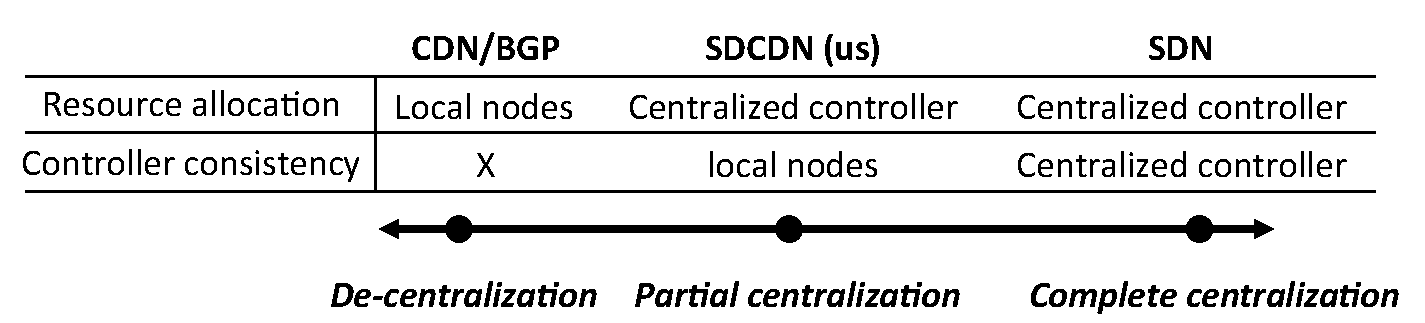
\includegraphics[width=1.0\columnwidth]{figures/design-space-3.pdf}
\caption{Design choices}
\label{fig:design-space}
\end{figure}


Figure~\ref{fig:design-space} compares the different design choices of SDN (e.g., Onix), CDN, and \SDCDN in two dimensions, i.e., resource allocation and consistency control. Unlike SDN or current CDNs which completely rely on local or centralized decision, SDCDN performs these functionalities in both controller and distributed servers.

	\myparatight{Resource allocation} Since the centralized controller is not sufficient for real-time decision, the resource allocation in SDCDN is done in two time scales. The controller performs global coordination with less constraints on real-timeness and produces {\it hint}s to each server. The local control process performs real-time resource allocation (e.g., path selection) based on the hints of global control process. Therefore, the hints and real-time use of them becomes critical in balancing the global optimality and responsiveness in real time (as discussed in Section~\ref{?}).

	\myparatight{Controller inconsistency} We let multiple controllers (i.e., global control processes) make decisions independently, and each server will receive multiple and possibly inconsistent decisions of controllers. SDCDN relies on servers to resolve the inconsistency if it exists, and merge them into a final decision used by data plane. Therefore, it is critical merge these decisions in a fashion that more fresh decisions are preferred but with less instability (as discussed in Section~\ref{?}).

Figure~\ref{fig:design-space} also depicts the spectrum of design space from de-centralization to complete centralization.  When projecting related systems onto this spectrum, current CDNs and SDNs are closer to the decentralization and centralization end respectively, and our design of SDCDN is in the middle of what we call {\it partial centralization}.
Although the concept of partial centralization of system design itself is not an innovation and it has been used for years (e.g., \cite{?}), our contribution is to exploit its potential benefits in implementing a control plane for wide-area overlay networks through a customized design in CDN environments.









\section{Design}

\begin{comment}
\subsection{Components}
Overview of whole system and functionalities of each component. 

\subsection{Interfaces}
Introduce forwarding table (between data plane and control plane), hint (within control plane between controller and nodes), NIB (between discovery modules and control plane)

\subsection{Flexible Data plane}
Our data plane can be based on existing proxy servers (e.g., Apache server) used by production networks. What flexibility we need from data plane.
\begin{itemize}
	\item Understand and execute based on the forwarding table.
	\item Provide information for in-band passive measurement.
\end{itemize}

\subsection{Discovery}
Discovery consists of local process running on each node to output local NIB, and global process that combines the local NIBs to output a global NIB.

\begin{itemize}
	\item how to compute global NIB from local NIBs
	\item when to inform global control process of a change in global NIB to prevent frequent recalculating (when it is converged?) \jc{need some idea...}
\end{itemize}

\subsection{Control plane}
The control plane design has three parts: global control process, local control process, and merging algorithm.

Global control process: globally coordinated resource share. output global hint based on application-level goals. Coarse time granular.

Local control process: detect connection failure/congestion from local NIB and output local hint.

Merging algorithm: merge global hint from multiple controllers and local hint. need to meet requirements: (i) correctness, and (ii) prefer local hint when local hint strongly suggests current forwarding table is hopeless.
\end{comment}


\begin{figure*}[t]
\centering
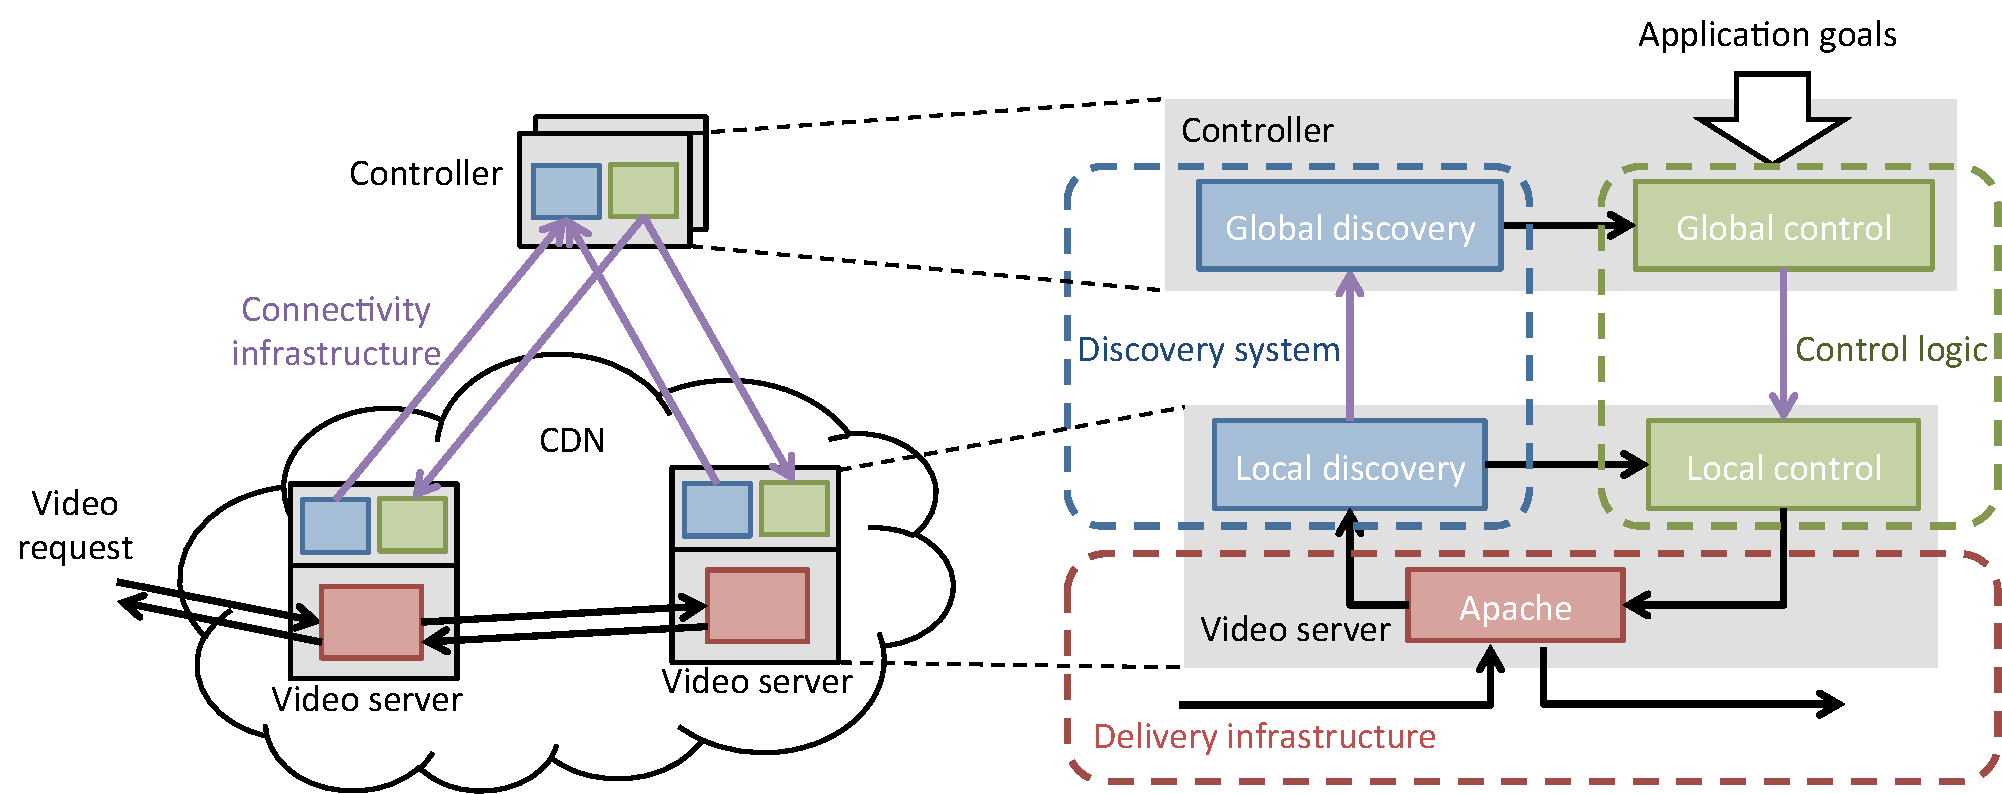
\includegraphics[width=2.0\columnwidth]{figures/system-overview-2.pdf}
\caption{System overview of SDCDN.}
\label{fig:system-overview}
\end{figure*}

This section first gives an overview of the components of a software-defined CDN (\SDCDN) and then presents the design choices and implementation of each components. 

\subsection{Overview of \SDCDN}

There are five components in  (see Figure~\ref{fig:system-overview}). 

\myparatight{\Data} This includes servers as well as any other network elements (such as cache) that perform content delivery and support an interface to measure and control the forwarding state. For simplicity, we call such nodes servers in \data. In live video streaming, the \data consists of several video origin server and a set of intermediate and edge servers that forward the content request to the origin server or a cached replica and deliver the requested content back.

\myparatight{\Dissemination} This communication between servers and the centralized controller transits the \dissemination. It must support bidirectional communication -- collecting statistics from servers to the controllers and disseminating decisions from the controllers to servers, and optionally support specific protocols to enforce receiving order of messages.

\myparatight{\Discovery} The \discovery runs both on servers and controllers. Local process of \discovery running on each server gathers statistics on both network states (e.g., link failure) and application information (e.g., which streams are more popular) through the measurement interface provided by \data. It then sends the summarized result to \localControl (as discribed below for real-time adaptation) and the controller through \dissemination. The global process of \discovery in the controller collects the network states and application information, and generates a network information base (NIB) and stream information base (SIB) respectively.

\myparatight{\GlobalControl} \GlobalControl performs joint optimization to coordinate network resource and video streams based on NIB and SIB generated by \discovery. The result of \globalControl is in form of a hint to each server that specifies for the request of each stream a set of next hop servers. The \globalControl has customized logic to support application-level goals (e.g., video quality optimization).

\myparatight{\LocalControl} \LocalControl receives hints from multiple controllers and measurement from local process of \discovery, and performs real-time control on the behavior of \data. 



\subsection{\Data}

The \data consists of video servers that perform content delivery for a wide range of protocols. We use HTTP as the basic transport protocol. Although traditional belief is that UDP or other propriatory protocols are better than HTTP because they reduce the latency, streaming live video over HTTP has recently been developed and advocated by industry in various protocols (e.g., \cite{HLS, HDS}) and standards \cite{dash}. The driven force of this trend is that HTTP has better middlebox support than other protocols and is well supported by CDNs to delivery web contents.

\mypara{Support multi-bitrate chunk-based live streaming with standard web servers}

\mypara{Forwarding table} map between a stream prefix and a forwarding strategy (forward the request to next hops by specified probability distribution and specified timeout). introduce format: stream prefix, set of next hops, timeout

\begin{figure}[h]
\centering
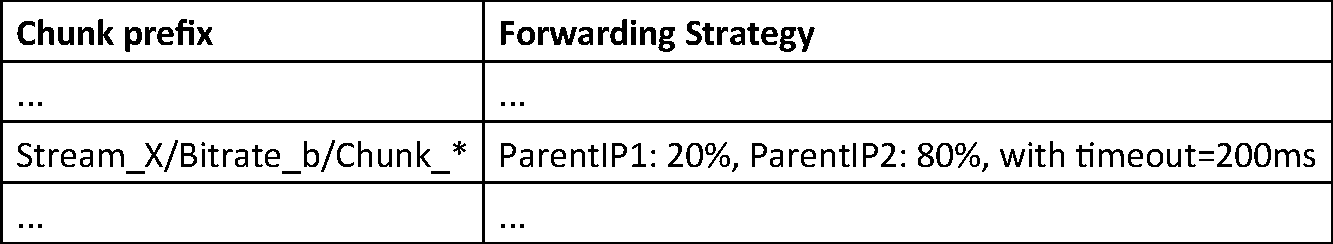
\includegraphics[width=1.0\columnwidth]{figures/forwarding-table-format.pdf}
\caption{Forwarding table}
\label{fig:forwarding-table}
\end{figure}

\mypara{Control interface} 
\begin{itemize}
	\item Implement forwarding table
	\item For a time-out request, change to another destination.
\end{itemize}

\mypara{Measurement interface}
\begin{itemize}
	\item Request received
	\item Request time-out
	\item Request download time, downloaded size
	\item Request for unknown request
	\item Request from unexpected interface
\end{itemize}

\mypara{Integration with standard HTTP web server} 
\begin{itemize}
	\item What Apache already provides (request count, loop detection, cache, timeout, multi-path): why is future-proof
	\item Integration issues
\end{itemize}



\subsection{\Dissemination}

The \dissemination maintains the communication between controller and servers. It is used by both \discovery and \decision. 

\begin{itemize}
	\item Design choices: in-band vs. out-band, point-to-point vs. multicast protocol. Our implementation uses RPyC: out-band and point-to-point (why)
	\item Deal with connection failure. Notify sender after timeout
	\item Traffic aggregation at egress/ingress of cluster. 
\end{itemize}


\subsection{\Discovery}

The goal of \discovery is to maintain a global on network states and stream states based on the information collected from measurement interface of \data. Network states include the network topology, performance of links within and between clusters of video servers.  Stream states include statistics of each video stream  (e.g., number of requests). We use two data structures, network information base (NIB for shor) and stream information base (SIB for short) to store the network states and stream states separately.

The basic entity of network state can be the pysical links or overlay links between two servers depending on the visibility of the measurement method. In this work, we use passive in-band measurement that measures throughput of video delivery between two servers, and thus the network state consists of throughput of all used overlay link.  Active measurement is also viable through cooperation between local monitoring processes running on different servers, and can discover more information, for example, physical link topology (via traceroute). However, these are out of our scope. \jc{Where to get topology information?}

A local monitoring process in each server collects local measurement results from measurement interface of \data and generates local NIB and SIB. Both need to be with timestamps. 

The local NIB and SIB will be sent back via \dissemination to the global monitoring process in controller periodically. These local NIBs and SIBs will be merged to update the global NIB and SIB.

The NIB and SIB are used to activate \decision when a significant change is detected in NIB or SIB. In real-time, if local SIB indicates a chunk request has timed out, the \localControl will be immediately activited and perform real-time reaction (for example, redirect the request to another neighbor). The global NIB and SIB are updated in a coarser time scale. When one or more links depart too much from its previous performance, it will initiate the \globalControl.

New stream establishment is also done by \discovery.

Finally, the traffic initiated by \discovery scales with more servers and more frequent, which places heavy burden on both \dissemination and \decision. Several widely used technique in SDN can be leveraged cluster-based traffic aggregation~\cite{?} and incremental update~\cite{?} to improve scalability.



\subsection{\Decision}

The \decision runs in both the controllers and servers, and makes decisions in three time scales.

\myparatight{Global coordination} The \globalControl in controllers is activated by global NIB and SIB generated by \discovery, makes decision of the forwarding strategy on each server for each stream, and sends the decision to each server by \dissemination. Such global decision is a soft control called global {\it hint}, based on which the \localControl decides forwarding table in real-time. \jc{Format of hint}

\myparatight{Realtime coordination} \localControl makes realtime coordination using two separate logics -- the {\it local decision algorithm} and the {\it merging algorithm}. The local decision algorithm gets triggered by local NIB and SIB and generates a local hint. On receiving any of local hint or global hint from one controller, the merging algorithm merges the newest version of local and global hints to update forwarding table in \data.

\myparatight{Application goals} The \decision also provides the flexibility in changing its logics to meet various application level goals. For example, the \decision can be configured to optimize for video quality (weighted sum of satisified bitrate) or bandwidth cost per cluster. In doing so, we must support runtime modification to the logics in both \globalControl and \localControl (local decision and merging algorithm). One possible approach is to write these logics in scripts which are called by another process that support runtime replacement of these scripts.











\section{Properties}

\subsection{Dissemination consistency}

\begin{itemize}
	\item Inconsistency of multiple versions of same controller: formulate the problem, introduce the solution
	\item Inconsistency of different controllers: formulate the problem, introduce the solution
\end{itemize}


\subsection{Fault tolerance}

Two stages after failure happens: local decision loop, and global decision loop


\subsection{Application-level quality improvement}
\begin{itemize}
	\item Example way to express quality and cost requirement
	\item Example algorithm to solve them
\end{itemize}

\section{Evaluation}


\section{Related work}



\section{Conclusion}

{\footnotesize \bibliographystyle{acm}
\bibliography{../common/bibliography}}


\theendnotes

\end{document}







